\chapter{QR factorisation}

\section{QR-Zerlegung}
\subsubsection{Definition}
Eine Matrix $A \in \mathbb{R}^{m \times n}$ , $m \ge n$ besitzt eine eindeutige QR-Zerlegung.
\begin{align}
	A = QR
\end{align}
mit einer orthogonalen Matrix $ Q \in \mathbb{R}^{m \times n} $ und einer oberen Dreiecksmatrix $ R \in \mathbb{R}^{n \times n}$ 

% TODO Quelle suchen das ist von Wikipedia -.-

\subsubsection{QR Anwendung oder so was}
-LGS 
-Ausgleichsprobleme 
-QR-Verfahren 

\section{Householdertransformation}
\begin{figure} 
	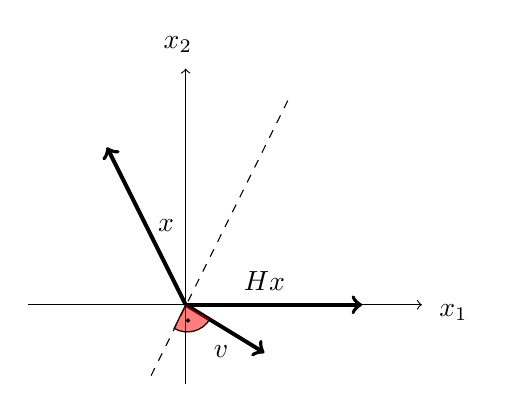
\begin{tikzpicture}

\draw[->] (-2,0) -- (3,0);
\draw[->] (0,-1) -- (0,3);

\draw[->,line width=0.5mm] (0,0) -- (-1,2);
\draw[->,line width=0.5mm] (0,0) -- (2.24,0);

\draw[dashed] (-0.44,-0.9) -- (1.34,2.68);
%\draw[->,line width=0.5mm] (0,0) -- (-0.9, 0.44);
%\draw[->,line width=0.5mm] (0,0) -- (-1,0.61);
\draw[->,line width=0.5mm] (0,0) -- (1,-0.61);





\filldraw[red, opacity=0.5] (0,0)--(-0.1467,-0.3000) arc (240:330:.3339) -- (0,0) ;
\draw[black, opacity=1] (0,0)--(-0.1467,-0.3000) arc (240:330:.3339) -- (0,0) ;
\filldraw(0.03,-0.2) circle (.02cm) ;

%Beschriftung
\draw (3.4,-0.1) node {$x_1$};
\draw (-0.1,3.3) node {$x_2$};

\draw (.45, -.6) node {$v$};
\draw (-.25, 1) node {$x$};
\draw (1,0.3) node {$Hx$};


\end{tikzpicture}
	\caption{Householder Trans}
	\label{fig:patrA}
\end{figure}
\subsection{Householder Vector}
\subsection{Apply vector}
\begin{align}
H =& I - \dfrac{vv'}{\tau}\\ 
H A_2 =& A_2 - \dfrac{vv'}{\tau}A_2\\
=& A_2 - \dfrac{v}{\tau}*(v'*A_2)
\end{align}

\section{LAPACK QR}
Der von LAPACK benutzte Algorithmus \cite{DGEQR2}
\begin{align}
	H &= I - \tau \omega \omega^T \\
	\tau &= \frac{\alpha - \beta}{\beta} \\
	\alpha &= A(i,i)\\
	\beta &= \text{sign}(\alpha) \left|\sqrt{\alpha^2 + \|x\|^2}\right|\\
	x &= A(i+1:m,i)\\
	\omega &= A(i+1:m,i) * \frac{1}{\alpha - \beta}
\end{align}
Algorithmus
\begin{lstlisting}
householderVektor(Vektor v, alpha, tau)
  beta = sign(sqrt(alpha ^2 + norm(x)^2),alpha)
  tau = (alpha - beta) / beta	
  scal(1/(alpha - beta), v)
\end{lstlisting}
\begin{lstlisting}
tau=zeros(min(m,n))
for i = 0 : min(m,n)
  householderVektor(A(i+1:m,i), A(i,i), tau(i)) 
  if (i < n && tau != 0)
    AII = A(i,i)
    A(i,i)= 1
    A = A - tau *w(w'*A) // MV und rank1
    A(i,i) = AII
\end{lstlisting}

\section{NUM1 Urban QR}
Algorithmus aus Numerik 1

Mathe
\begin{align}
	H &= I - 2 \frac{\omega \omega^T}{\omega^T \omega}\\
	\omega_1 &= \frac{x - \alpha e_1}{x_1 - \alpha}\\
	\alpha ^2 &= \|x\|^2 
\end{align}
Algorithmus
\begin{lstlisting}
householderVektor(Vektor x, omega, beta)
  n = length(x)
  if n> 1
    sigma = x(2:end)'*x(2:end);
    if sigma==0
      beta = 0;
    else
      mu = sqrt(x(1)^2+sigma);
      if x(1)<=0
        tmp = x(1) - mu;
      else
        tmp = -sigma / (x(1) + mu);
      end
      beta = 2*tmp^2/(sigma + tmp^2);
      x(2:end) = x(2:end)/tmp;
    end
    v = [1;x(2:end)];
  else
    beta = 0;
    v = 1;
  end
\end{lstlisting}

\begin{lstlisting}
for i = i:n
  housevector(A(i:m, i), w, beta)
  A(i:m,i:n) = (I(m-i+1) - beta * w * w')*A(i m,i:n)
  if i < m
    A(i + 1 : m, i) = w(2:m-i+1)
\end{lstlisting}

\section{Unterschiede der Algorithmen}
LAPCK hat das Tau \\
Vor und Nachteile oder so was

\section{QR Blocked}
Geblockte Alorighmus
\begin{align}
H &= I - VTV'\\
H' &= I - VT'V'\\ 
H'A_2 &= A_2 - VT'V'A_2
\end{align}

\begin{figure} 
	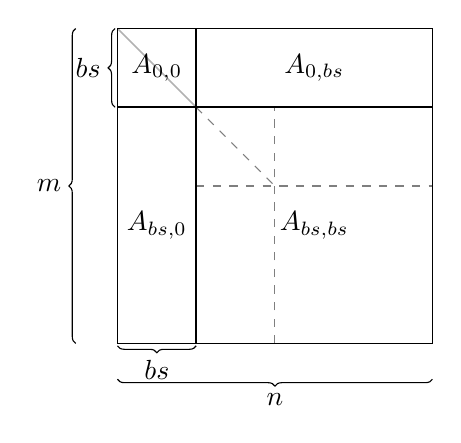
\begin{tikzpicture}
\draw[semithick] (0,0) -- (4,0) -- (4,4) -- (0,4) -- (0,0);

\draw[semithick] (1,0) -- (1,4);
\draw[semithick] (0,3) -- (4,3);
\draw[semithick,opacity=0.3] (0,4) -- (1,3);

\draw[dashed,opacity=0.5] (2,0) -- (2,3);
\draw[dashed,opacity=0.5] (1,2) -- (4,2);
\draw[dashed,opacity=0.5] (1,3) -- (2,2);


\draw (0.5,3.5) node {$A_{0,0}$};
\draw (0.5,1.5) node {$A_{bs,0}$};
\draw (2.5,3.5) node {$A_{0,bs}$};
\draw (2.5,1.5) node {$A_{bs,bs}$};
\draw[decorate, decoration={brace,mirror}, yshift=-.2ex]  (0,0) -- node[below=0.4ex] {$bs$}  (1,0);
\draw[decorate, decoration={brace}, xshift=-.2ex]  (0,3) -- node[left=0.4ex] {$bs$}  (0,4);
\draw[decorate, decoration={brace,mirror}, yshift=-3ex]  (0,0) -- node[below=0.4ex] {$n$}  (4,0);
\draw[decorate, decoration={brace}, xshift=-3.5ex]  (0,0) -- node[left=0.4ex] {$m$}  (0,4);

\end{tikzpicture}
	\caption{Partitionierung vom A}
	\label{fig:patrA}
\end{figure}





Betrachte A geblockt
\begin{align}
	A = \left(\begin{array}{l|l}
	A_{0, 0} & A_{0, \text{bs}} \\ \hline
	A_{\text{bs}, 0}   & A_{\text{bs}, \text{bs}} 	
	\end{array} \right) 
\end{align}

Berechne QR Zerlegung für Blöcke $A_{0, 0}$ und $ A_{\text{bs},0}$
\begin{align}
	\left(\begin{array}{l} 
	A_{0, 0} \\ \hline
	A_{\text{bs}, 0}
	\end{array}\right)
	\leftarrow
	\left(\begin{array}{l} 
	Q_{0, 0}  \backslash R_{0,0} \\ \hline
	Q_{\text{bs}, 0} 
	\end{array}\right)
\end{align}

Berechne $H(0)$...$H(bs)$ aus $Q_{0, 0}$ und $Q_{bs, 0}$ mit $H = I - V*T*V^T$.\\
Wende $H^T$ auf $A_{0, \text{bs}}$ und $ A_{0,\text{bs}}$ an.
\begin{align}
	\left(\begin{array}{l} 
	A_{0, \text{bs}} \\ \hline
	A_{0, \text{bs}}
	\end{array}\right)
	\leftarrow
	H^T \left(\begin{array}{l} 
	A_{0, \text{bs}} \\ \hline
	A_{0, \text{bs}}
	\end{array}\right)
\end{align}



Fahre mit $A_{0, \text{bs}}$ fort.

\subsection{Calc Factor T larft}
\cite{Joffrain:2006:AHT:1141885.1141886}

\begin{align*}
	H_2 H_1 x &= (I-\tau_2 v_2 v_2^T)(I-\tau_1 v_1 v_1^T)x\\
	&= (I - \tau_1 v_1 v_1^T - \tau_2 v_2 v_2^T - \tau_2 v_2 v_2^T \tau_1 v_1 v_2^T) x\\
  &= x - \tau_1 v_1 v_1^T x - \tau_2 v_2 v_2^T x - \tau_1 \tau_2 v_2 (v_2^T v_1 )v_2^T x\\
  &= x - \tau_1 v_1 v_1^T x - \tau_2 v_2 v_2^T x - \tau_1 \tau_2 (v_2^T v_1 ) v_2 v_2^T x\\
\end{align*}

\begin{align*}
  H_{1,2} x &= (I - V T V^T) x = x - V T V^T x\\
  &= x - (v_1, v_2)
  \begin{pmatrix}
    a & b \\ 0 & c
  \end{pmatrix}
  \begin{pmatrix}
    v_1^T \\ v_2^T 
  \end{pmatrix}
  x\\
  &= x - (v_1, v_2)
  \begin{pmatrix}
    a & b \\ 0 & c
  \end{pmatrix}
  \begin{pmatrix}
    v_1^T x \\ v_2^T x
  \end{pmatrix}\\
  &= x - (v_1, v_2)
  \begin{pmatrix}
    a v_1^T x + b v_2^T x\\  c v_2^T x
  \end{pmatrix}\\
  &= x - v_1(a v_1^T x + b v_2^T x) - v_2 (c v_2^T x)\\
  &= x - a v_1 v_1^T x - b v_1 v_2^T x - c v_2 v_2^T x
\end{align*}

\subsection{Apply H larfb}
Die Funktion larfb berechnet.

\begin{align}
	H^T A &= A - V T^T V^T A
\end{align}

\begin{figure} 
	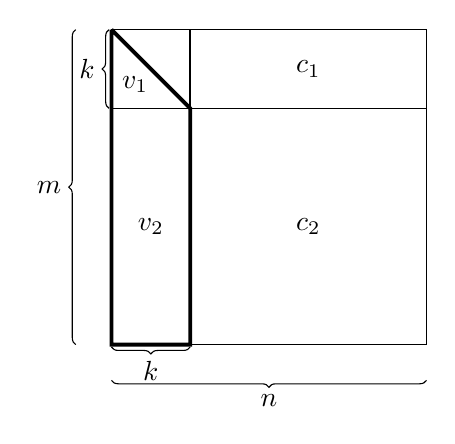
\begin{tikzpicture}
\draw[semithick] (0,0) -- (4,0) -- (4,4)-- (0,4)-- (0,0);


\draw[semithick] (1,0) -- (1,4);
\draw[semithick] (0,3) -- (4,3);
\draw[line width=0.5mm] (0,4) -- (0,0) -- (1,0) -- (1,3) -- (0,4);


\draw[decorate, decoration={brace,mirror}, yshift=-.2ex]  (0,0) -- node[below=0.4ex] {$k$}  (1,0);
\draw[decorate, decoration={brace}, xshift=-.2ex]  (0,3) -- node[left=0.4ex] {$k$}  (0,4);
\draw[decorate, decoration={brace,mirror}, yshift=-3ex]  (0,0) -- node[below=0.4ex] {$n$}  (4,0);
\draw[decorate, decoration={brace}, xshift=-3ex]  (0,0) -- node[left=0.4ex] {$m$}  (0,4);

\draw (0.3,3.3) node {$v_1$};
\draw (0.5,1.5) node {$v_2$};
\draw (2.5,3.5) node {$c_1$};
\draw (2.5,1.5) node {$c_2$};



\end{tikzpicture}
	\caption{Partitionierung vom A}
	\label{fig:patrA}
\end{figure}


\subsection{Iterativer Algorithmus}

\begin{algorithmic}
\For {i = 0 : n}
	\State QR = A;
	\If {i + ib > n}
		\State Calc T: H=I-VTV'
		\State Apply H: A=H'A
	\EndIf
\EndFor

\end{algorithmic}


\subsection{Rekursiver Algorithmus}


